\documentclass{article}
\usepackage[utf8]{inputenc}
\usepackage[english]{babel}
\usepackage[textheight=10in]{geometry}
\usepackage{amsmath}
\usepackage{amssymb} 
\usepackage[]{amsthm}
\usepackage{graphicx}
\usepackage{subfig}
\usepackage{float}
\usepackage{enumitem}
\setlist{  
  listparindent=\parindent,
  parsep=0pt,
}
\graphicspath{{../screenshots/}}

\begin{document}
\begin{enumerate}
	\item The constraints are: 
				\begin{enumerate}
					\item $P(d) <= 0.991058$
					\item $P(t | \bar d) <= 0.002332$
					\item $P(\bar t | d) <= 0.005966$
				\end{enumerate} \
		\begin{figure}[H]
			\centering
			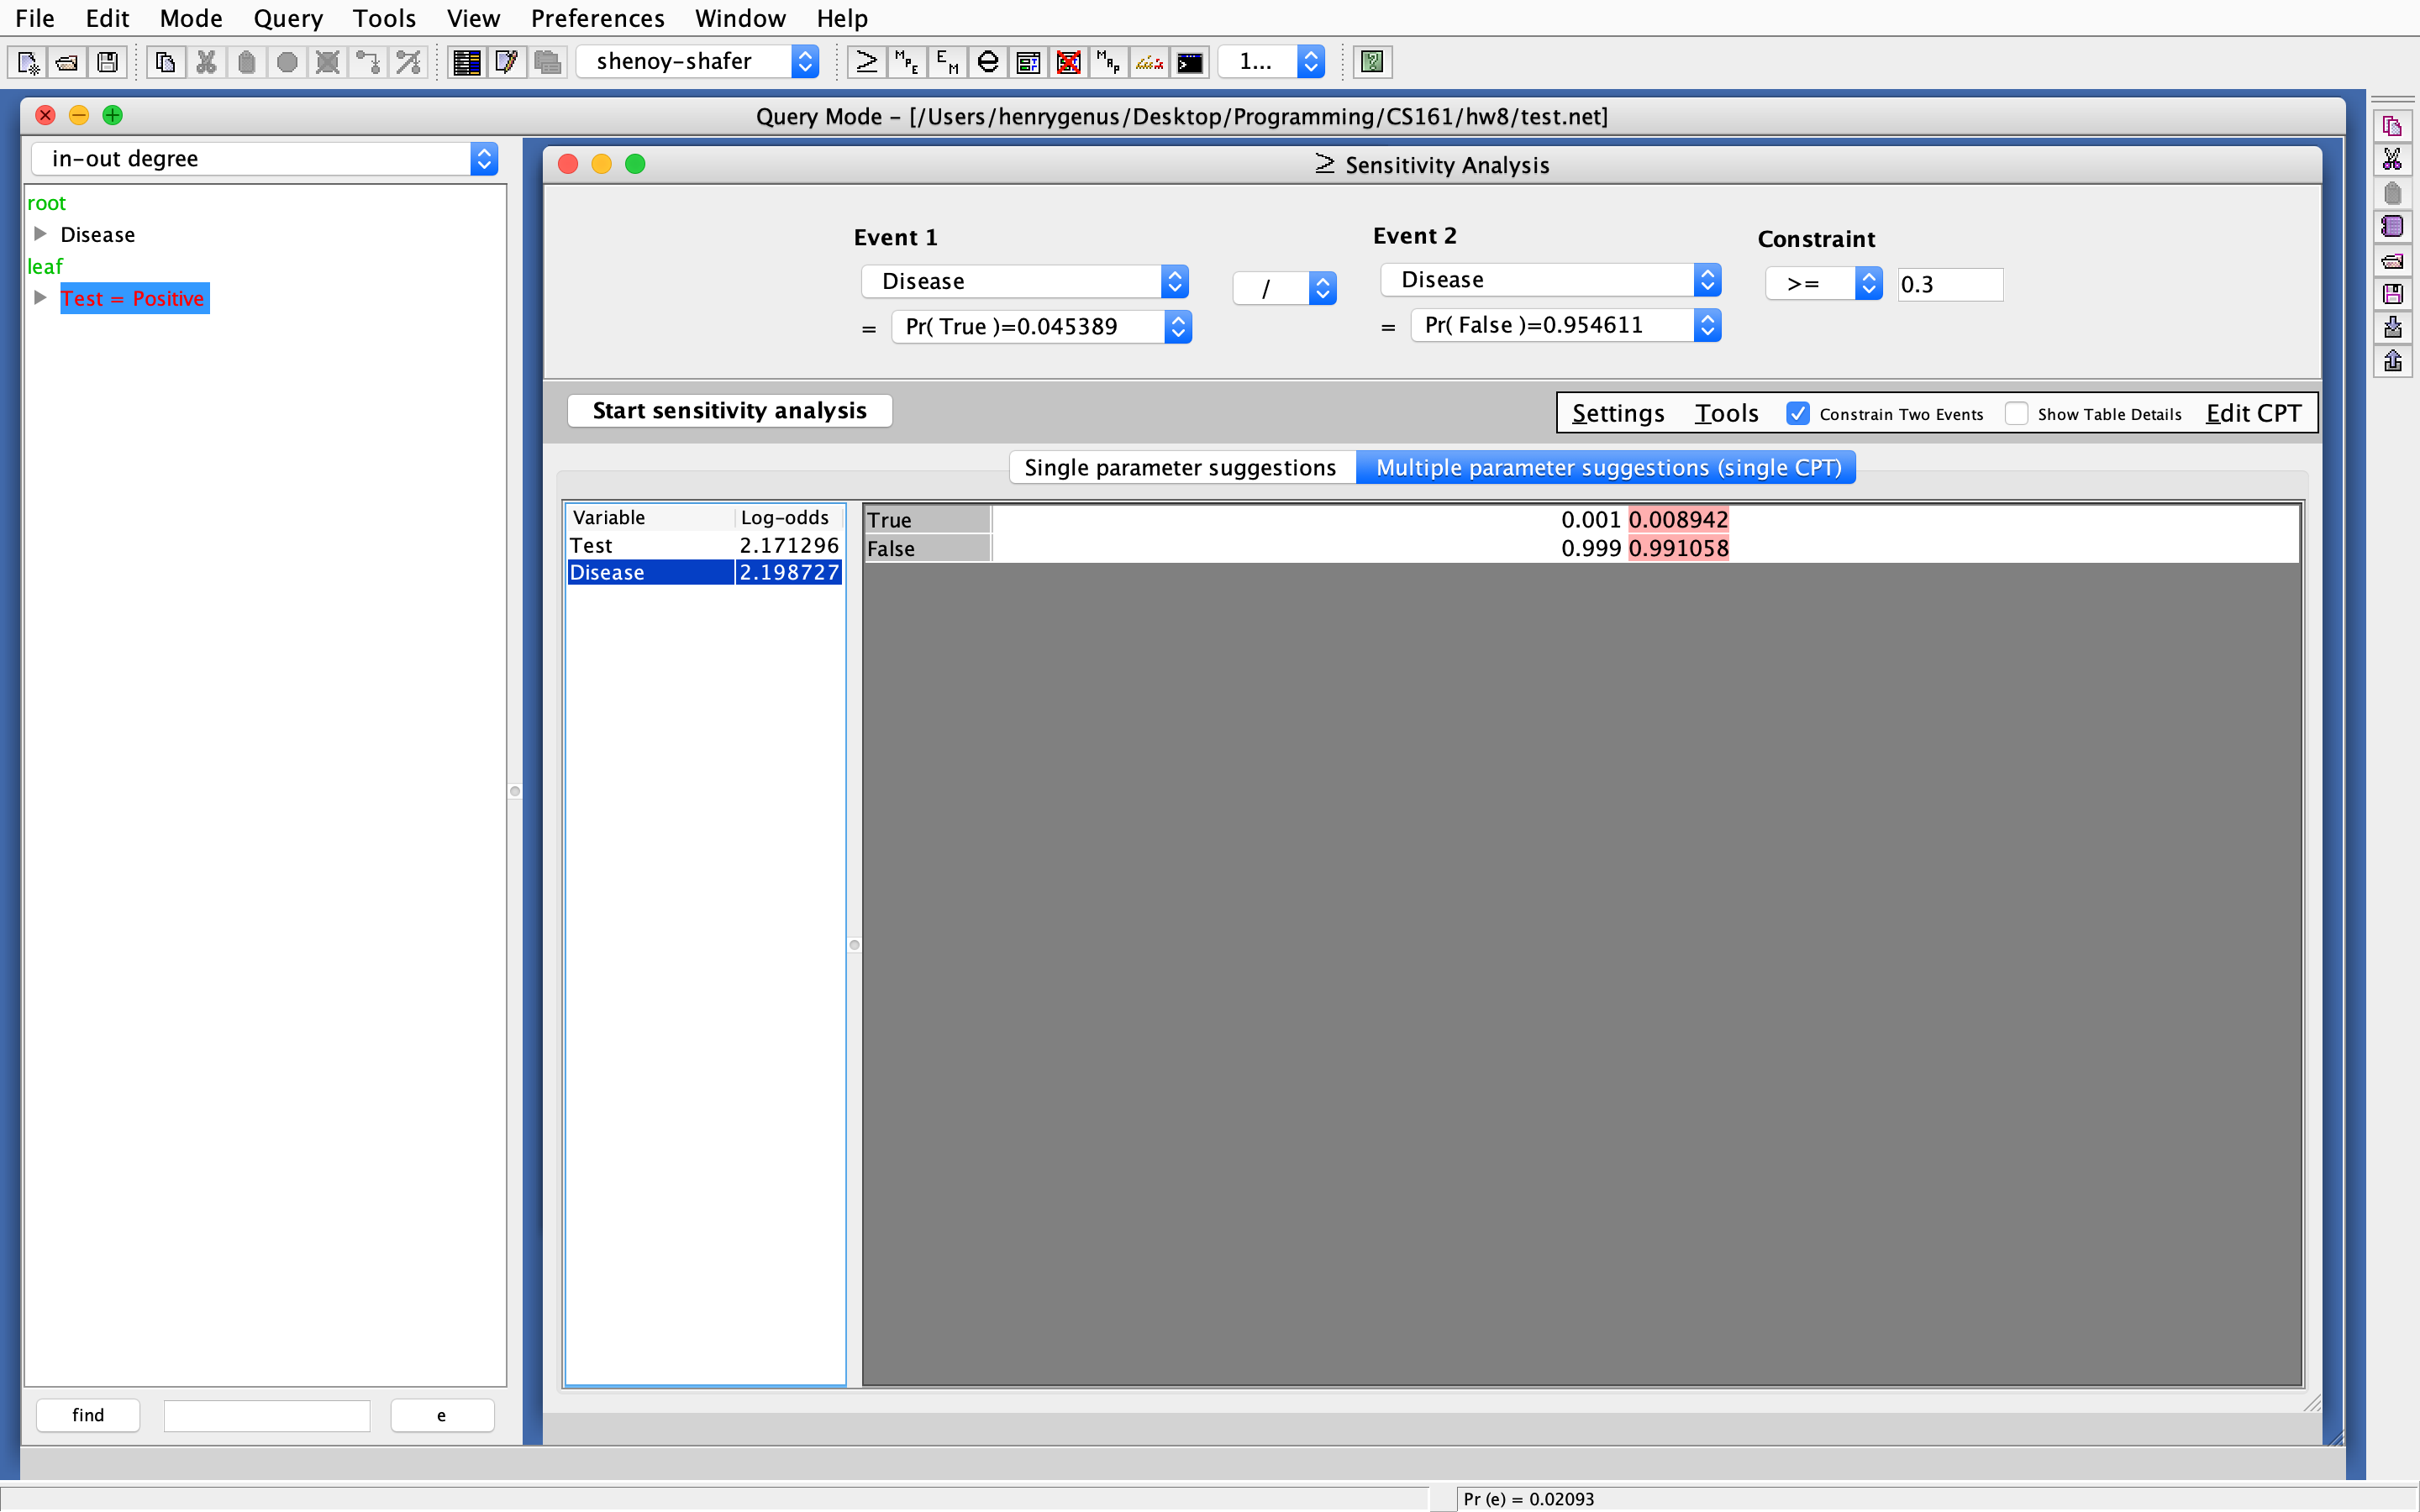
\includegraphics[width=\linewidth]{diseaseweight.png}
			\caption{Disease Constraint}
			\label{fig:dis}
		\end{figure}
		\begin{figure}[H]
			\centering
			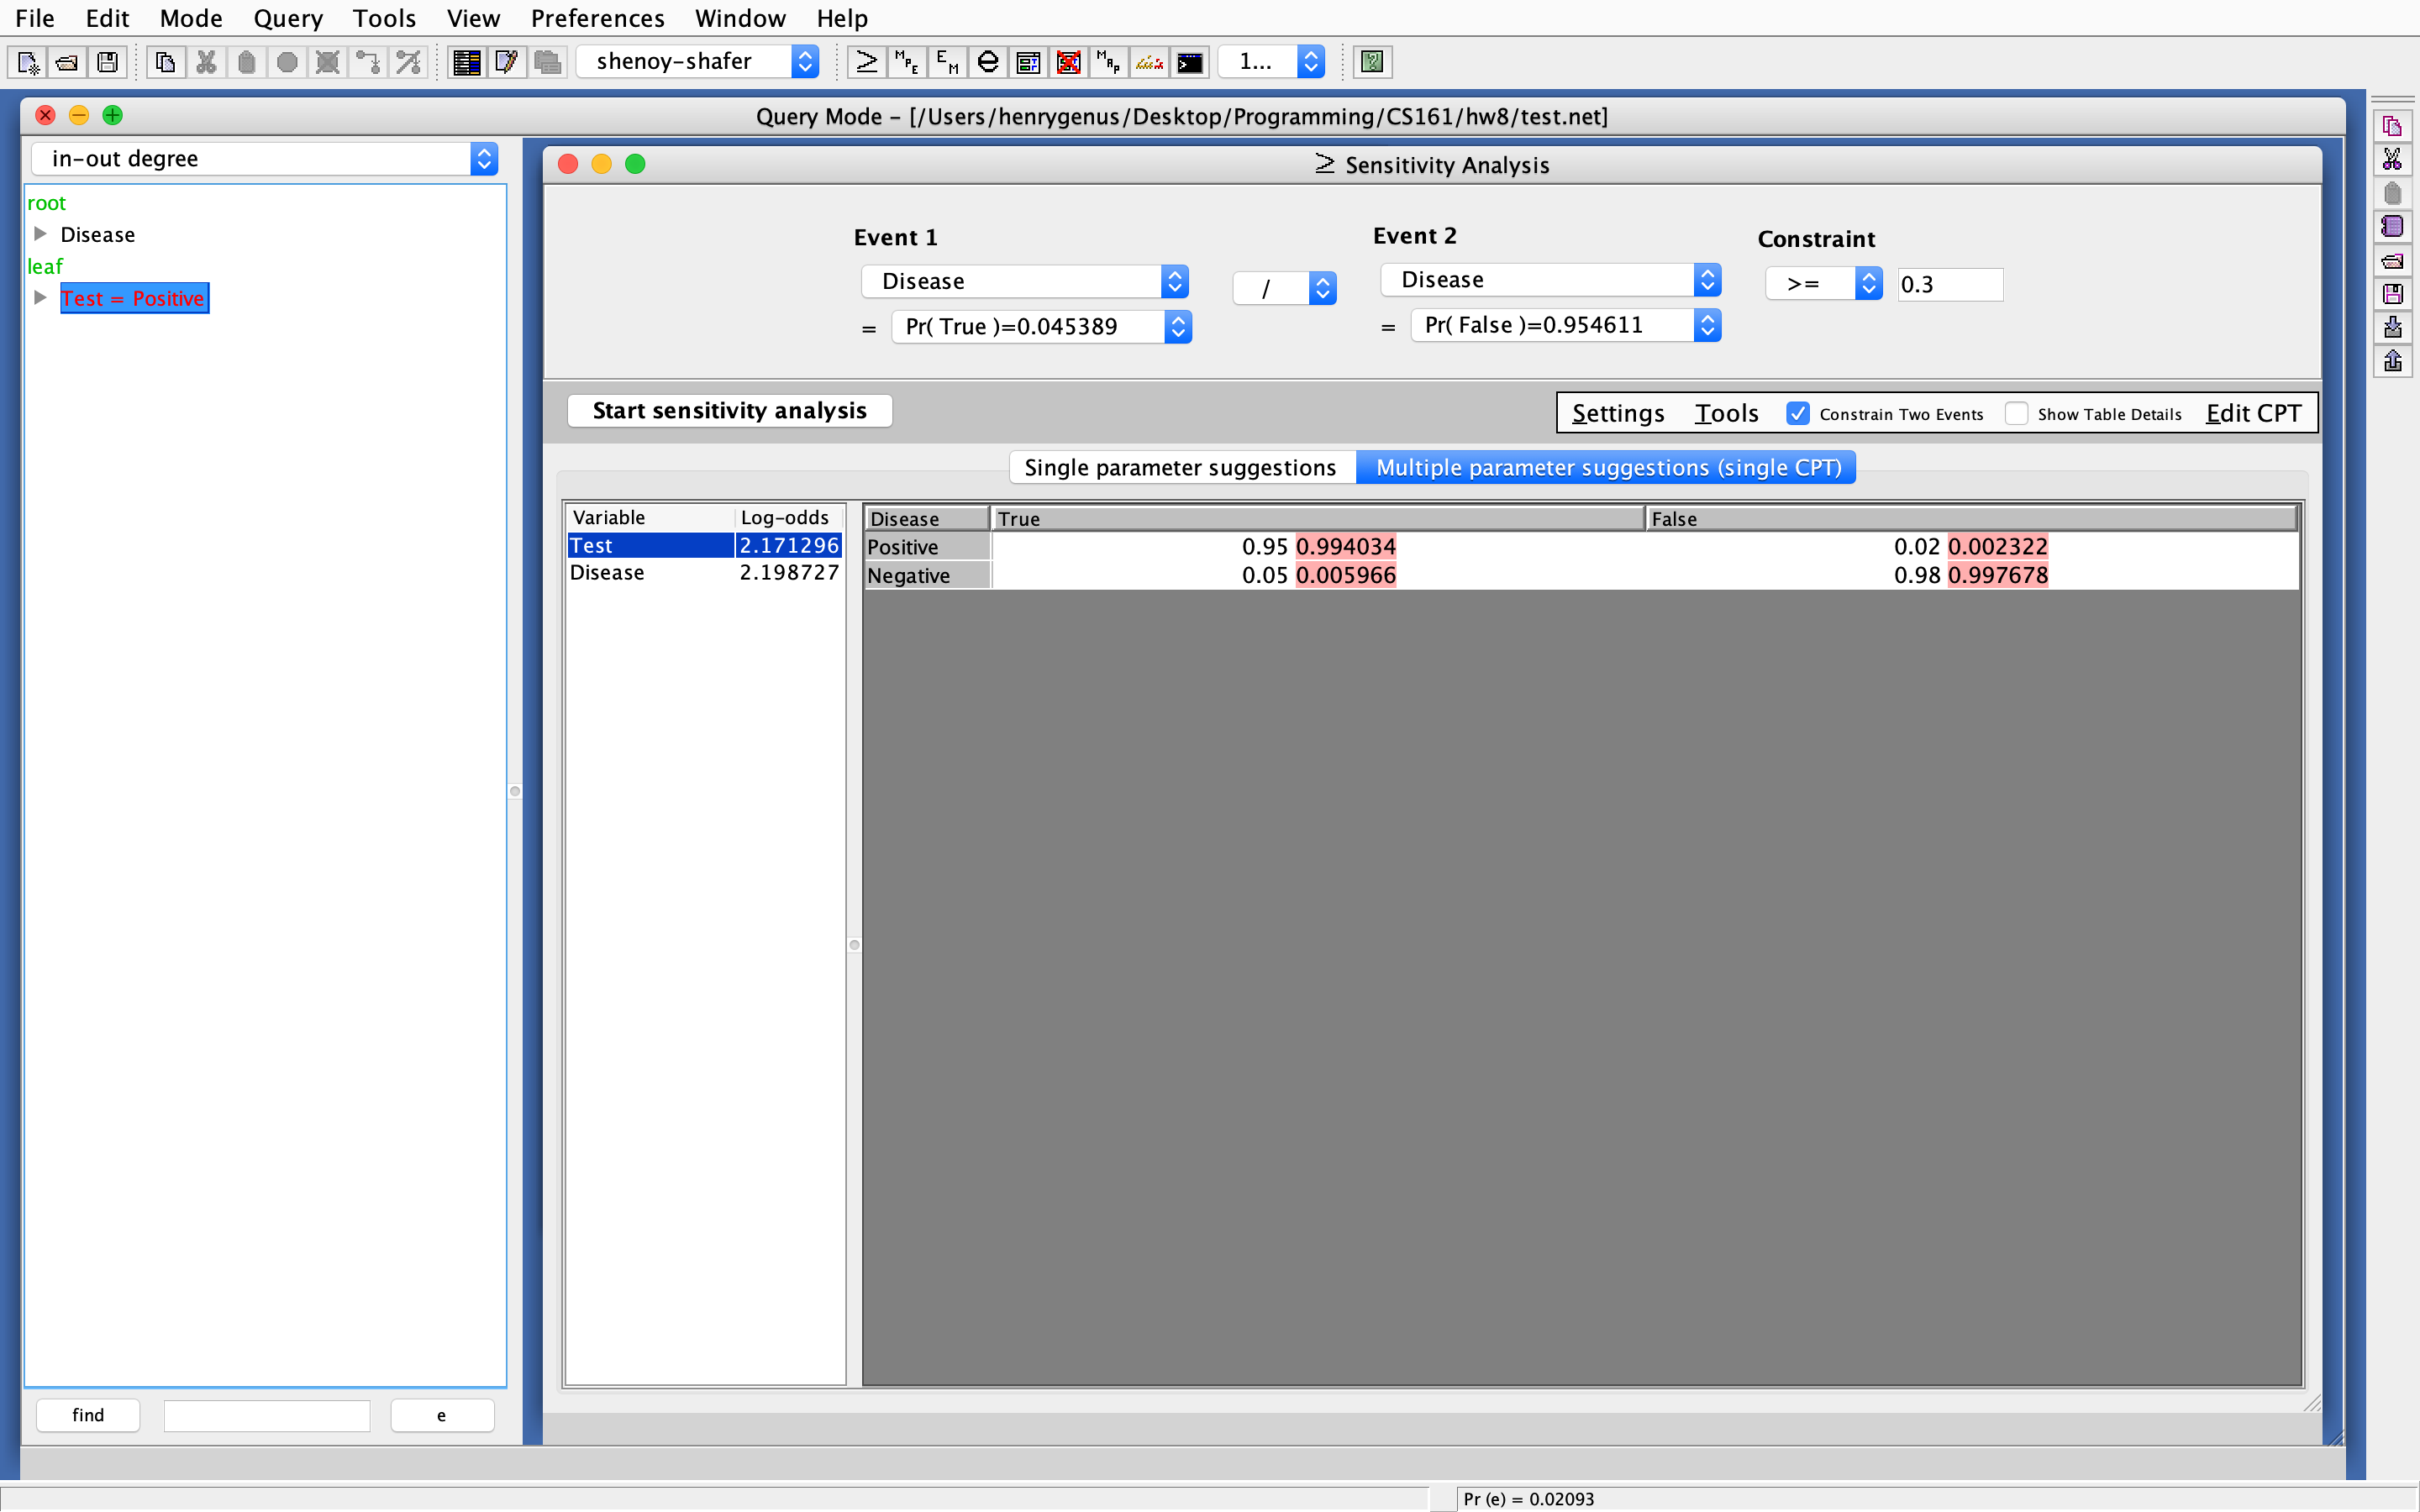
\includegraphics[width=\linewidth]{testweight.png}
			\caption{Test Constraints}
			\label{fig:test}
		\end{figure}
	\clearpage
	\item \begin{enumerate}
			\item MLE $|$ LightSensor $\land \ \neg$SoundSensor = \{\\
				\indent Battery = OK, \\
				\indent Dog Barking = No, \\
				\indent Dog Bowel Trouble =Yes, \\
				\indent Dog Outside = Yes, \\
				\indent Expecting Guests = No, \\
				\indent Family Home = No, \\
				\indent Hearable Barking = No, \\
				\indent Light Sensor Health = OK, \\
				\indent Outdoor Light = On, \\
				\indent Sound Sensor Health = OK \\
				\} \\
				Setting LightSensor and $\neg SoundSensor$ and using the MPE
					tool on the network gave us the following:
				\begin{figure}[H]
					\centering
					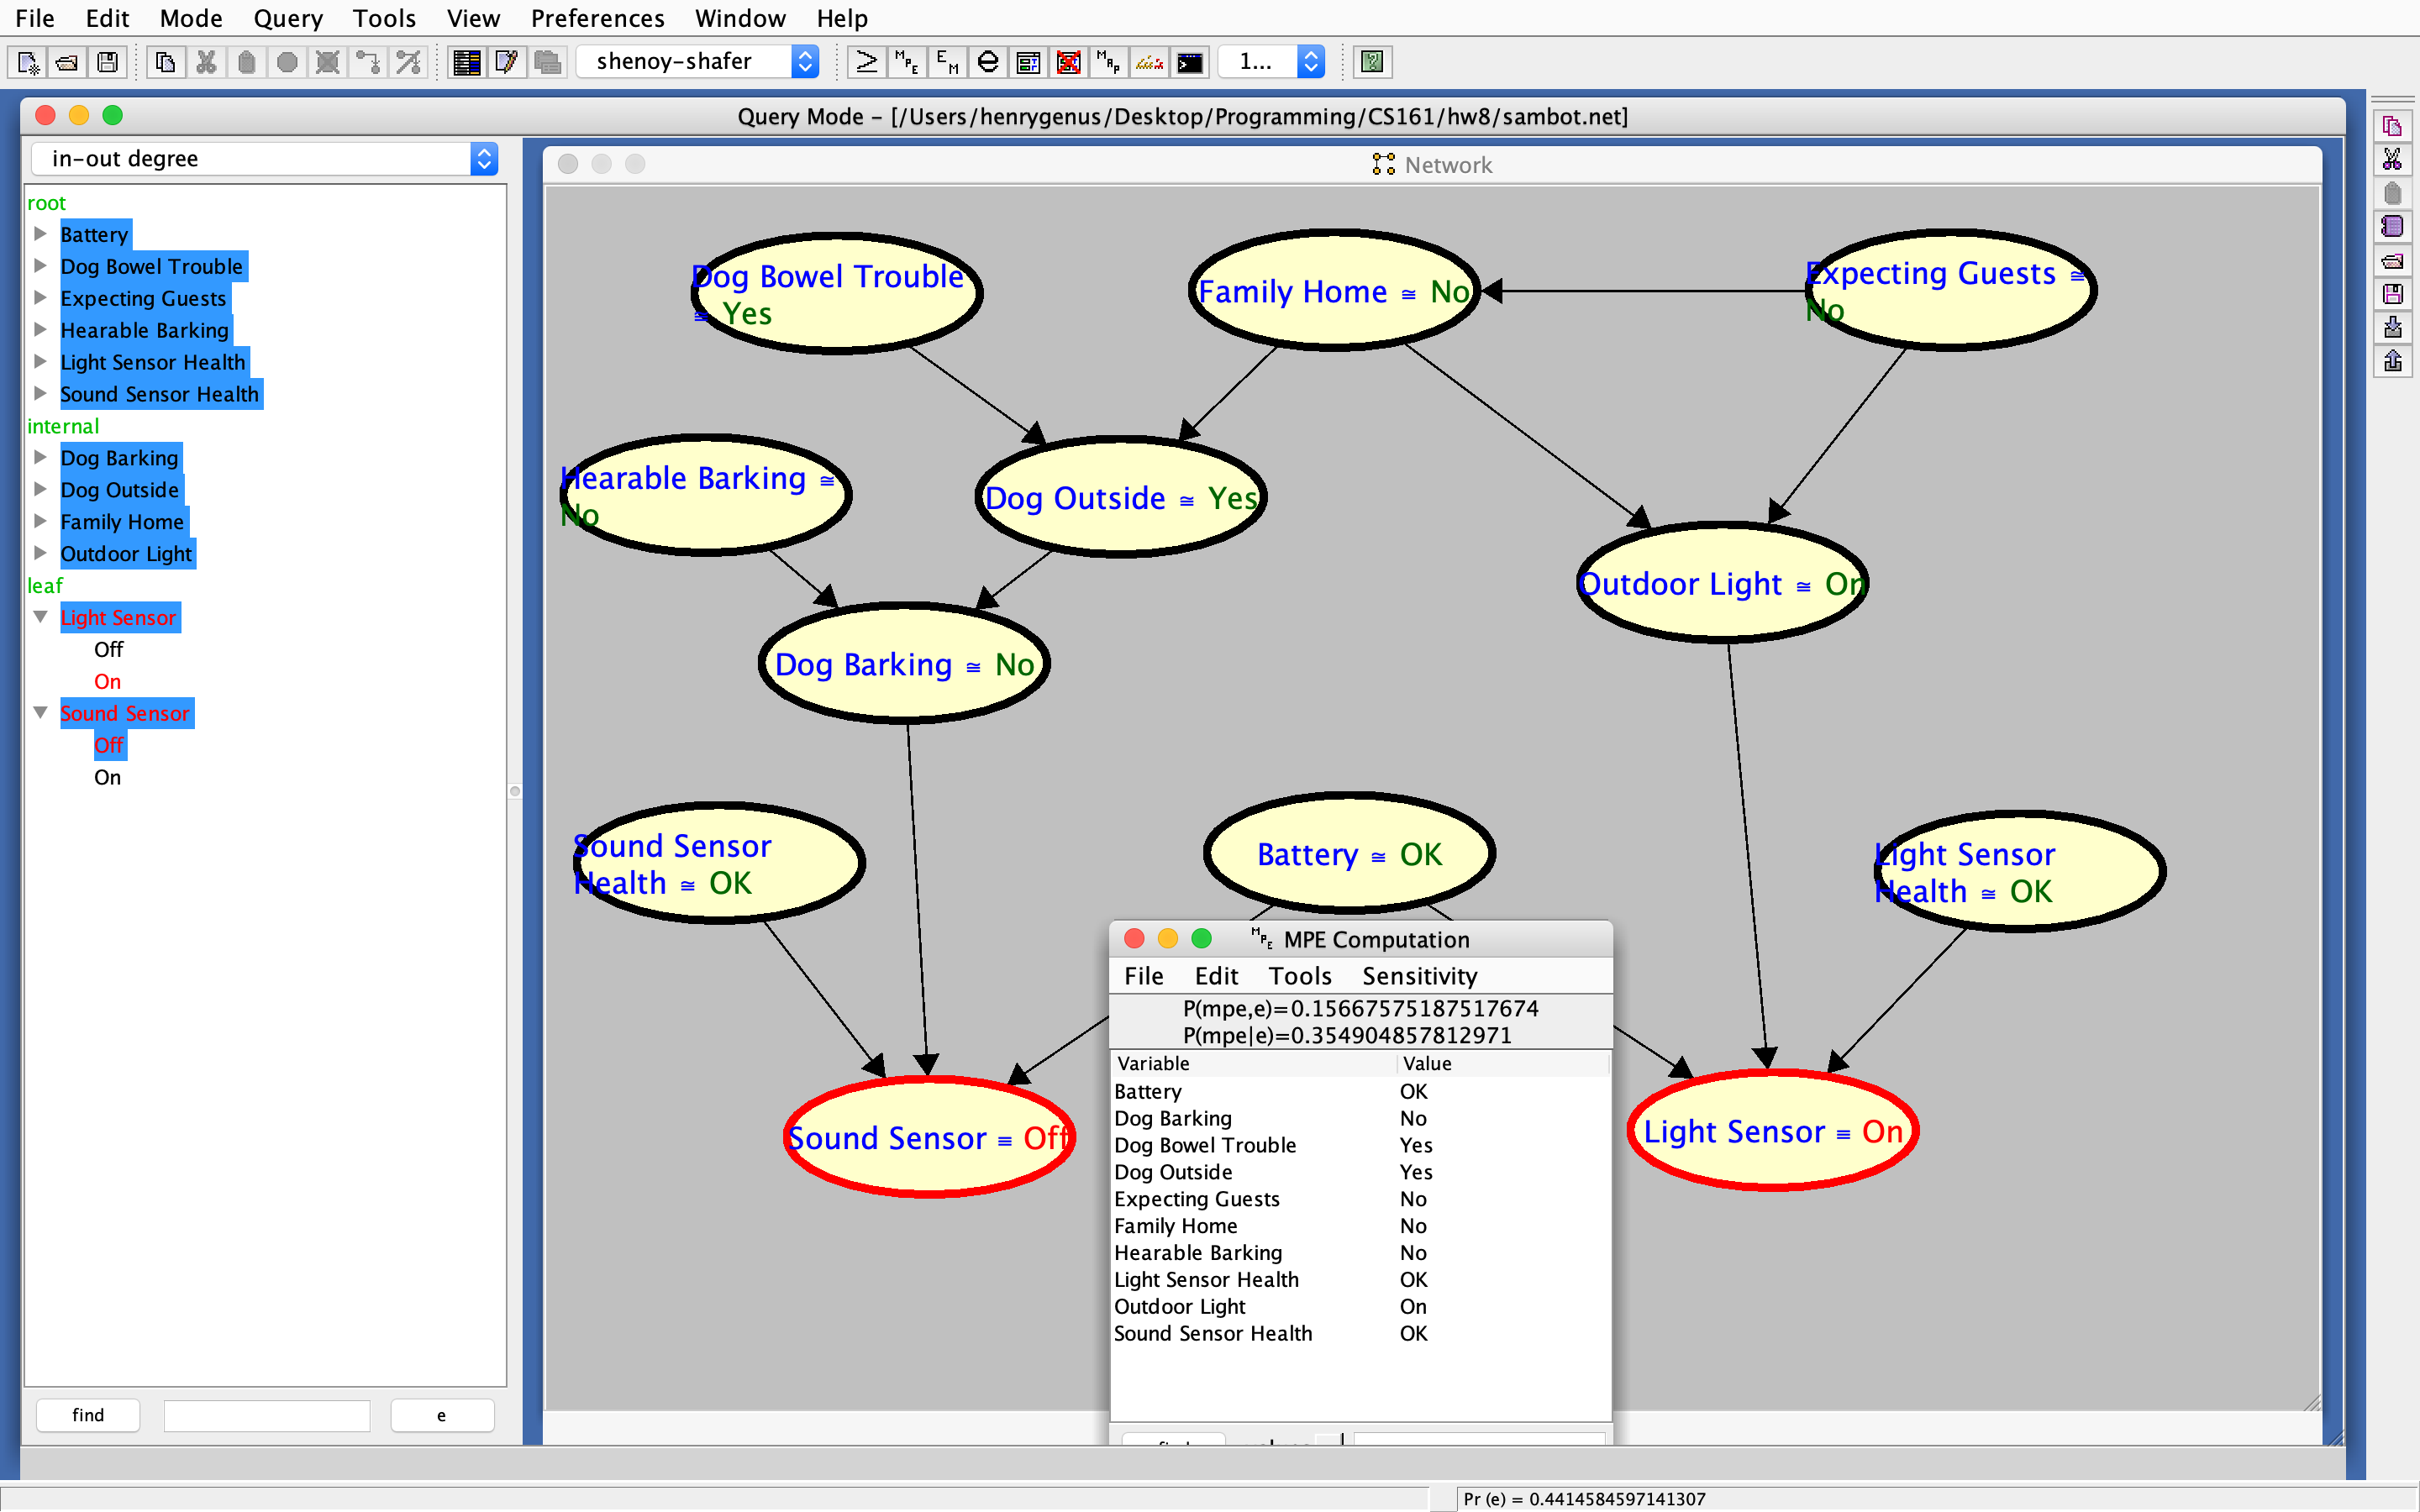
\includegraphics[width = \textwidth]{MPE_LS~BS.png}%
					\caption{MLE $|$ LightSensor $\land \ \neg$BarkSensor }
					\label{fig:L~B}
				\end{figure}
			\clearpage
			\item MLE LightSensor, SoundSensor 
					$|$ FamilyHome $\land \ \neg$ExpectingGuests = \{\\
				\indent LightSensor = Off, \\
				\indent SoundSensor = Off, \\
				\} \\
				Setting FamilyHome and $\neg$ExpectingGuests and using the MPE
					tool on the network gave us the following:
				\begin{figure}[H]
					\centering
					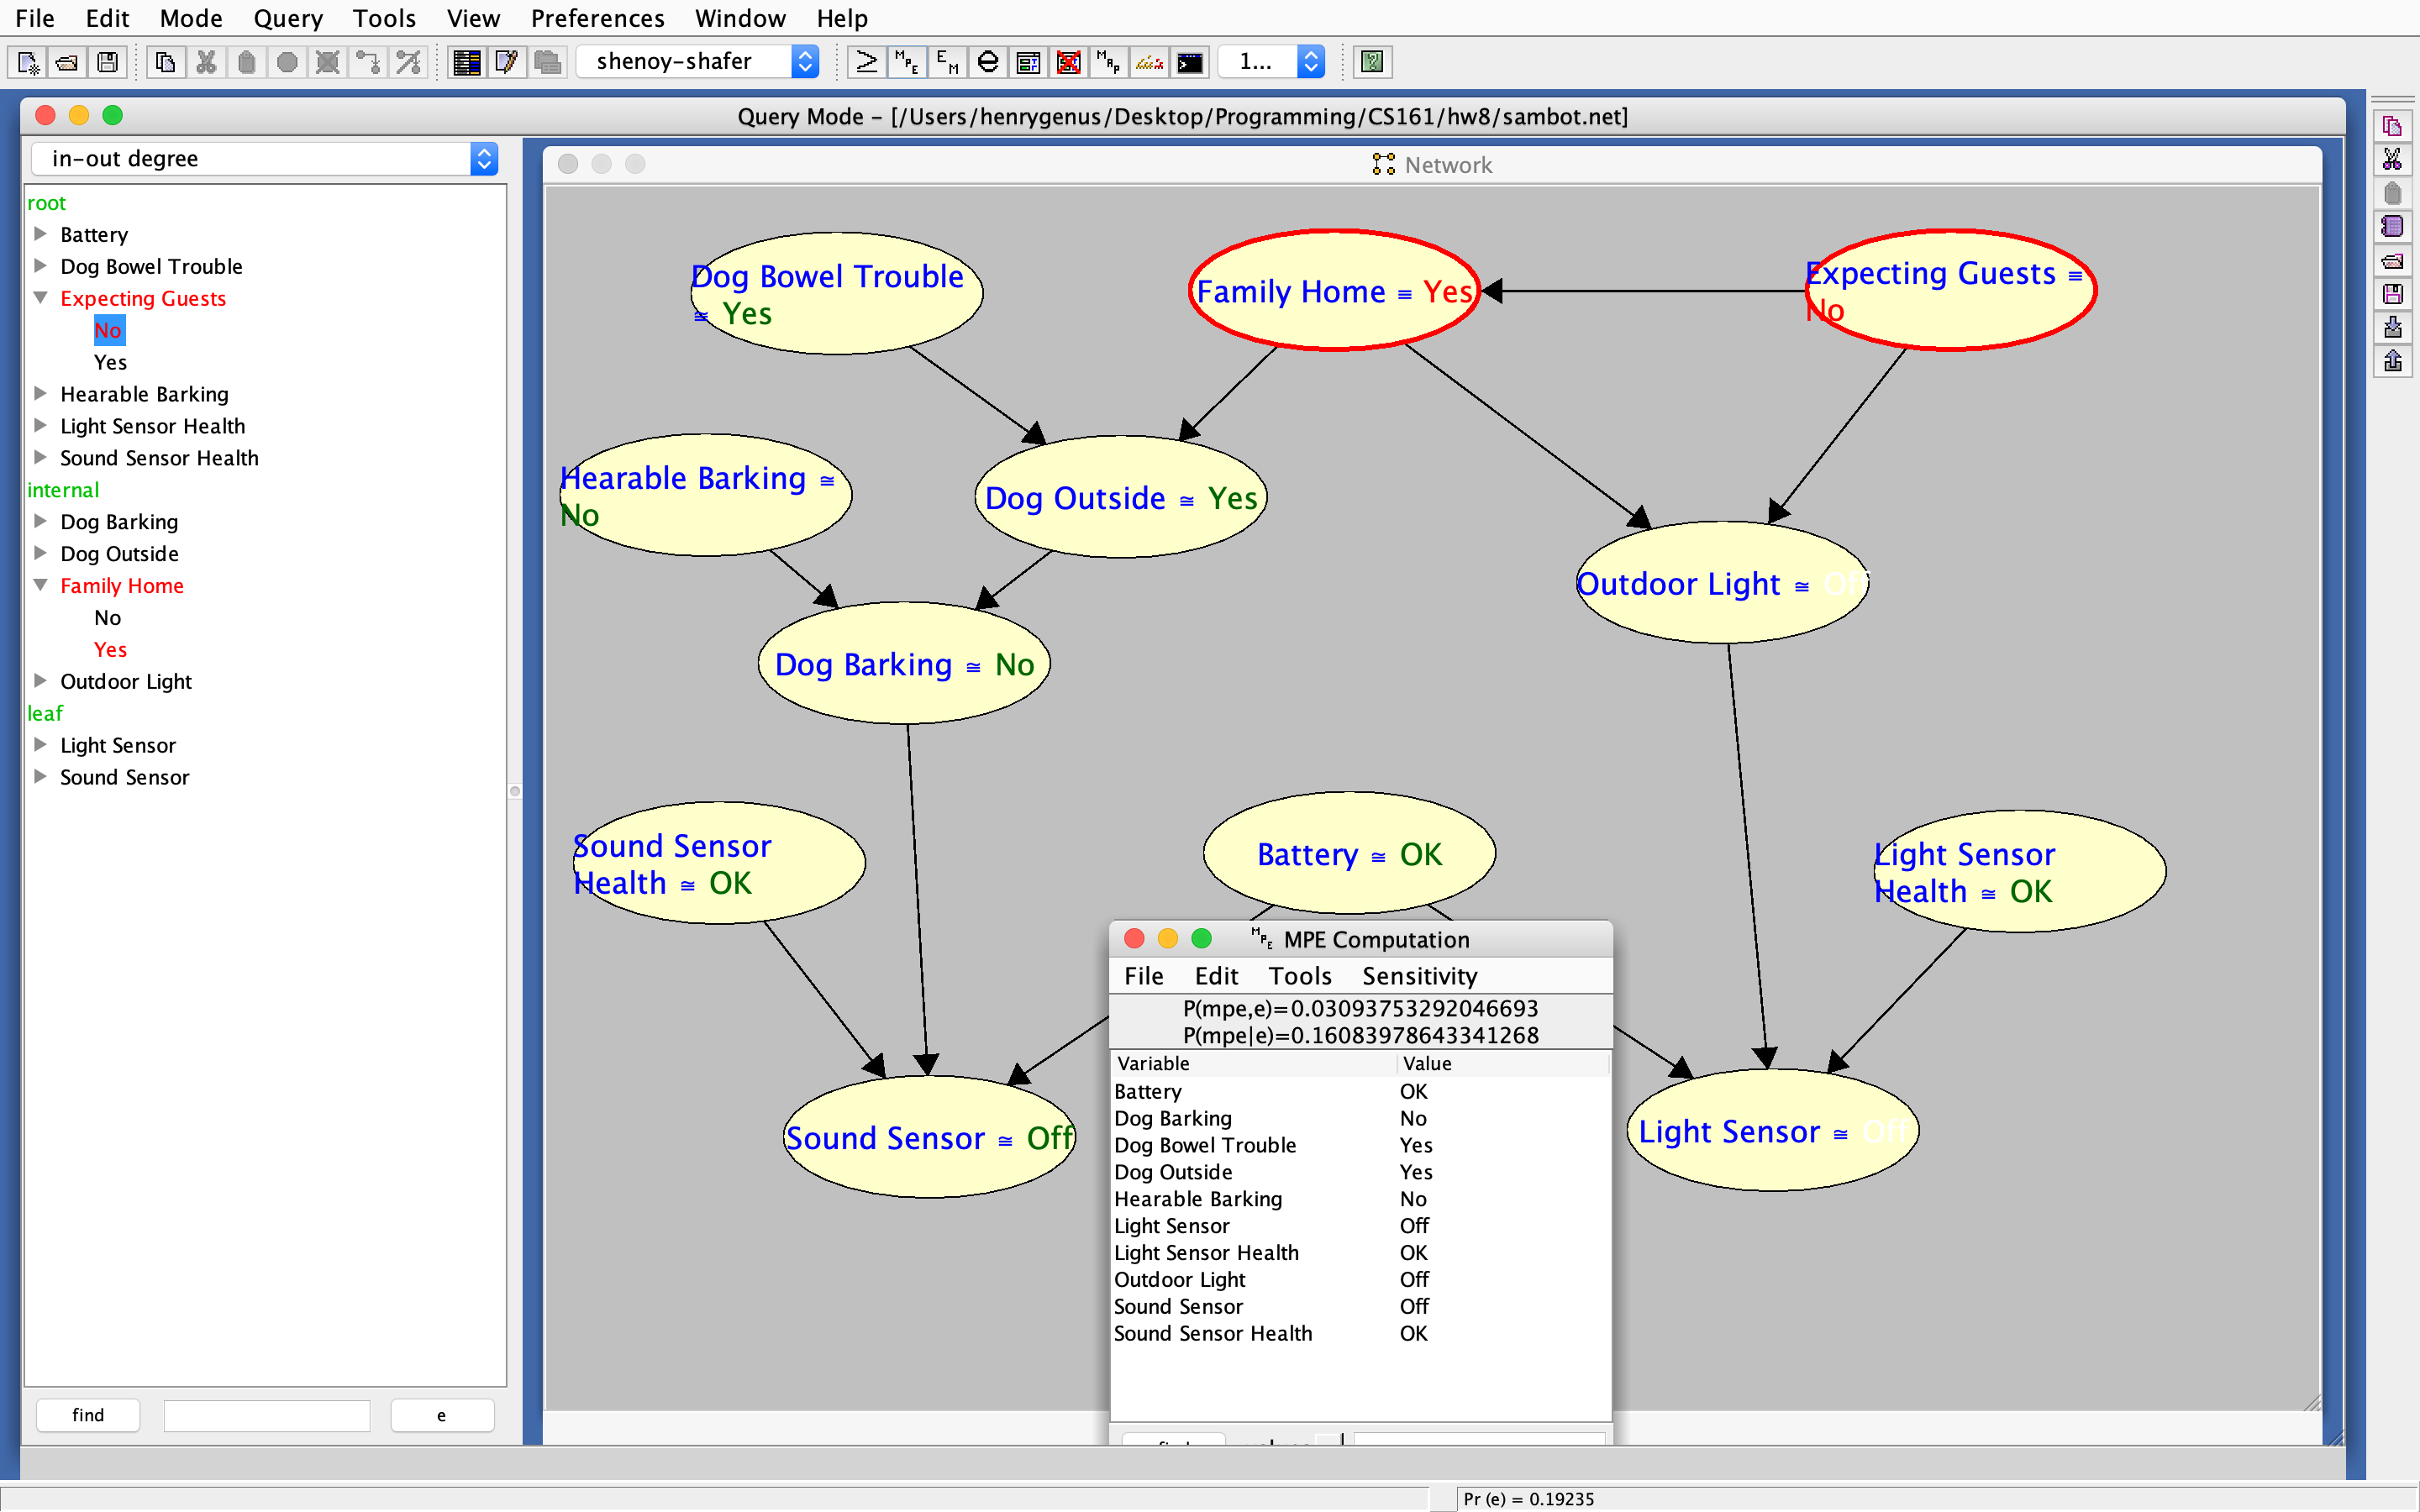
\includegraphics[width = \textwidth]{MPE_FH~EG.png}%
					\caption{MLE $|$ FamilyHome $\land \ \neg$ExpectingGuests}
					\label{fig:F~G}
				\end{figure}
			\item \begin{equation*}
					\text{MIN(\textbf{Z}) |  ND(SoundSensor, \textbf{Z}, LightSensor) 
					= \{Battery, FamilyHome\}} 
				\end{equation*}
			 \begin{proof}		
				We can see this by considering that all paths from SoundSensor to 
				LightSensor must flow through one of the two items in \textbf{Z}. \\
				
				Battery is divergent, so it blocks all paths through it. therefore \\
				\begin{equation*} 
					\text{blocked(SoundSensor, Battery, LightSensor)=True}
				\end{equation*}
				FamilyHome has two paths through it: \{ExpectingGuests, FamilyHome, 
				DogOutside\} and \{OutdoorLight, FamilyHome, 
				DogOutside\}.  The former is sequential and the latter is divergent,
				so both are blocked by assigning FamilyHome.  Therefore\\
				\begin{align*} 
					\text{blocked(ExpectingGuests, FamilyHome,  DogOutside)=True} \\ 
					\text{blocked(OutdoorLight, FamilyHome,  DogOutside)=True	}
				\end{align*}
				Thus we can see that\\ 
				\begin{equation*}
					\text{d\_SEP(SoundSensor, FamilyHome Battery, LightSensor)=True}
				\end{equation*}
				and therefore that\\
				\begin{equation*}
					\text{IND(SoundSensor, FamilyHome  Battery, LightSensor)=True.}
				\end{equation*}
				\end{proof}
			\item Our structure is multiply connected, as can be seen by the triangular 
				connection of FamilyHome, ExpectingGuests, and OutdoorLight, 
		\end{enumerate}
	\end{enumerate}
\end{document}